%\usetikzlibrary{patterns}
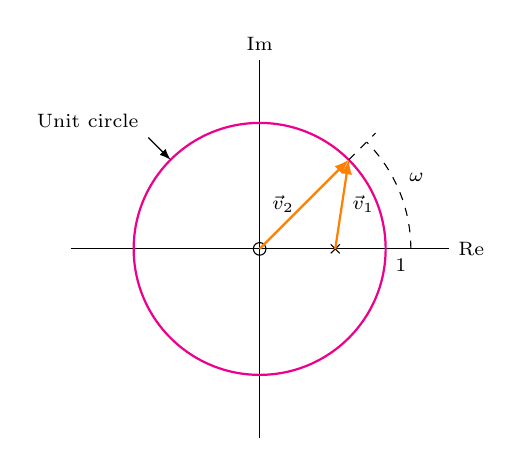
\begin{tikzpicture}[scale=0.8]
    \def\pole{++(135:0.1) -- ++(-45:0.2) ++(135:0.1) -- ++(45:0.1) -- ++(-135:0.2) +(45:0.1)}
    \def\zero{circle (0.1)}

    \draw (-3, 0) -- (3,0) node[anchor=west] {\scriptsize $\mathrm{Re}$};
    \draw (0, -3) -- (0,3) node[anchor=south] {\scriptsize $\mathrm{Im}$};
    %\pause
    \draw[thick, magenta] (0,0) circle (2);
    \draw [latex-] (0,0) ++(135:2) -- ++(135:0.5) node [anchor=south east] {\scriptsize Unit circle};
    \node at (2, 0) [anchor=north west] {\scriptsize $1$};

    %\node at (2, 1) [anchor=west] {\scriptsize $z$-plane};
    \coordinate (p1) at (0:1.2);
    %\coordinate (p2) at (-60:1.5);    
    \coordinate (o) at (0,0);
    \coordinate (a) at (45:2);
    \draw (p1) node[anchor=north east] {} \pole;
     %\draw (p2) node[anchor=north east] {} \pole;
    \draw (0,0) \zero;
    %\draw (0,0) circle (0.07);
    
    
    \draw[dashed] (o) -- (p1);
    %\draw[dashed] (o) -- (p2);    
    \draw[dashed]  (45:2) -- ++(45:0.6);
    \draw[-latex, thick, orange] (p1) -- (a) node [midway, black, anchor=west] {\scriptsize $\vec{v}_1$};
  \draw[-latex, thick, orange] (o) -- (a) node [midway, black, anchor=east] {\scriptsize $\vec{v}_2$};       
  %\draw[-latex, thick, orange] (p2) -- (a);         
  
  \draw[dashed] (2.4,0) arc (0:45:2.4)  node [midway, anchor=south west] {\scriptsize $\omega$};    ;
 % \draw (0.6,0) arc (0:-60:0.6);  
  %\node at (20:0.8) {\scriptsize $\theta$};
  %\node at (-20:0.8) {\scriptsize $\theta$};  
   %\node at (a) [anchor=south west] {\scriptsize $\Omega=\theta$};    

\end{tikzpicture} 